% DoseRAD2026 final paper, based on Springer's official LLNCS samplepaper.tex
% (LLNCS package version 2.21, 2022/01/12).
\documentclass[runningheads]{llncs}

\usepackage[T1]{fontenc}
\usepackage{graphicx}
\usepackage{booktabs}
\usepackage{tabularx}
\usepackage{array}
\usepackage{xcolor}
\usepackage{url}
\usepackage[hidelinks]{hyperref}

\graphicspath{{figures/}}
\newcommand{\methodname}{ProtonFiLM-Lite}
\newcolumntype{Y}{>{\raggedright\arraybackslash}X}
\setlength{\textfloatsep}{10pt plus 2pt minus 2pt}
\setlength{\floatsep}{8pt plus 2pt minus 2pt}

\begin{document}

\title{Energy-Conditioned 3-D Residual U-Nets with 2.5-D UNet++ Synthetic CT for Proton Dose Prediction from CT and MRI}
\titlerunning{Residual U-Nets for Proton Dose Prediction from CT and MRI}

\author{C\'edric H\'emon\inst{1} \and Valentin Boussot\inst{2} \and
Jean-Claude Nunes\inst{1} \and Caroline Lafond\inst{1}}
\authorrunning{C. H\'emon et al.}
\institute{Univ. Rennes, CLCC Eug\`ene Marquis, INSERM, LTSI -- UMR 1099,
F-35000 Rennes, France
\and
Fideus Labs, Durham, NC 27713, United States}

\maketitle

\begin{abstract}
We describe one method for the DoseRAD2026 proton-dose tasks on computed
tomography (CT) and magnetic resonance imaging (MRI). Both tasks use the same
3.09-million-parameter, six-level residual 3-D U-Net on a beam's-eye-view
(BEV) grid of $288\times64\times64$ voxels at $2\times1\times1$~mm. Proton
energy is encoded by feature-wise linear modulation of deep network stages.
The final 80-epoch continuation used masked beam mean absolute error (MAE) plus
integrated depth-dose (IDD) distance, AdamW at $10^{-4}$, cosine annealing to
$4\times10^{-5}$, BF16 mixed precision, an effective batch of four, and paired
lateral flipping ($p=0.25$). Phase epoch 79 minimized the six-patient cached-BEV
validation objective at 0.010897 (MAE 0.006335; IDD 0.004561) and was retained
as the single dose checkpoint.
For MRI, one 26.08-million-parameter 2.5-D UNet++ with a ResNet-34 encoder first
maps five adjacent MR slices to synthetic CT (sCT). It was fine-tuned using
body-masked L1 plus $0.15$ times a SAM-based perceptual loss, AdamW, and
coherent spatial and MR-intensity augmentation. The best fold-1 checkpoint by
validation body MAE was retained. At inference, complete slices are processed
in FP16 batches of 16, converted to $[-1024,3071]$ HU, and set to air wherever
the original MR is exactly zero.
Order-3 cubic B-splines map anatomy to BEV and dose back to the native grid.
Predictions are non-negative and values at or below each beamlet's provided
minimum cutoff are zeroed; no upper clipping or ensemble is used. Native-space
dose metrics must still be recomputed for the final checkpoint. Independent
12-patient sCT validation gave body MAE
$51.995\pm14.756$ HU. A historical 176-beamlet HTTP profile of the same
architecture required 7.912~s; sCT generation averaged 1.265~s.

\keywords{Proton dose calculation \and residual U-Net \and synthetic CT \and magnetic resonance imaging \and beam's-eye view.}
\end{abstract}

\section{Introduction}

Accurate dose calculation is central to radiotherapy planning, but reference
Monte Carlo simulation remains computationally demanding. DoseRAD2026 provides
paired CT and MRI from thoracic and abdominal cases together with beam-level
Monte Carlo dose maps for photon and proton irradiation, enabling controlled
evaluation of learned dose engines~\cite{xiao2026doserad}. The proton tasks are
particularly sensitive to heterogeneous tissue composition because beam range
depends on the material traversed before the Bragg peak. MRI adds a second
difficulty: it provides valuable soft-tissue contrast but does not directly
encode the electron-density information normally derived from CT.

We entered the proton-on-CT and proton-on-MRI task variants. Our design
separates image-dependent geometry from beamlet-dependent inference. A compact
energy-conditioned residual 3-D U-Net predicts each beamlet in a fixed BEV
coordinate system. This reduces the spatial variability seen by the network
and permits the same dose model to process all proton energies and both
anatomical regions. MRI is handled by a preceding MR-to-sCT network rather than
by retraining the dose model directly on MR. This modular choice reuses the
same CT-calibrated dose mapping, while making the additional MR uncertainty and
latency explicit.

Our contributions are a compact energy-conditioned BEV dose model shared by
both tasks, a full-slice 2.5-D sCT route that avoids patch-stitching artifacts,
and an inference implementation that reuses spline coefficients and projected
anatomy across beamlets. We batch the 3-D network, perform cubic interpolation
on the GPU, overlap output compression with GPU work, and generate each sCT
only once. The final submission will use one dose and one sCT checkpoint;
ensembles were rejected when image-quality gains did not improve dose. We
report its training, internal validation, and runtime while distinguishing
model-selection data from independent and diagnostic evaluations.

\section{Methods}

\subsection{Data and validation splits}

The DoseRAD2026 data comprise 75 public training patients and 40 withheld test
patients, with 36 abdominal and 39 thoracic patients in the training cohort.
Each training patient has paired, geometrically aligned CT and MR volumes. The
proton subset contains 36 gantry angles, 15 rays per angle, and two sampled
energies per ray, or 1,080 beamlets per patient and 81,000 beamlets in total.
Native proton image and dose spacing is $1\times1\times3$~mm, and energies span
31.7290--200.7966~MeV~\cite{xiao2026doserad}. We used no additional dose
labels.

The final dose phase used 69 training patients and six model-selection
patients (1ABB039, 1ABB042, 1ABB061, 1THB008, 1THB120, and 1THB221; 6,480
beamlets). Four cases held out during development (1ABB135, 1ABB149, 1THB037,
and 1THB122) were added to final-phase training. Consequently, the earlier
ten-patient native-space analysis is not a held-out evaluation of the final
checkpoint.

The sCT fold used 63 training and 12 validation patients. Validation patients
were selected as six representatives per anatomy by K-means followed by the
nearest observed sample (medoid), using image dimensions, body/intensity
statistics, and beam geometry. Fold-1 validation cases were disjoint from its
63 training cases. The initialization was the public ImpactSynth MR--CBCT
CV-1 checkpoint, whose documented pretraining data include SynthRAD 2023 and
SynthRAD 2025 Task~1~\cite{boussot2025impact}; this is external pretraining and
is reported separately from DoseRAD fine-tuning.

\begin{figure}[t]
\centering
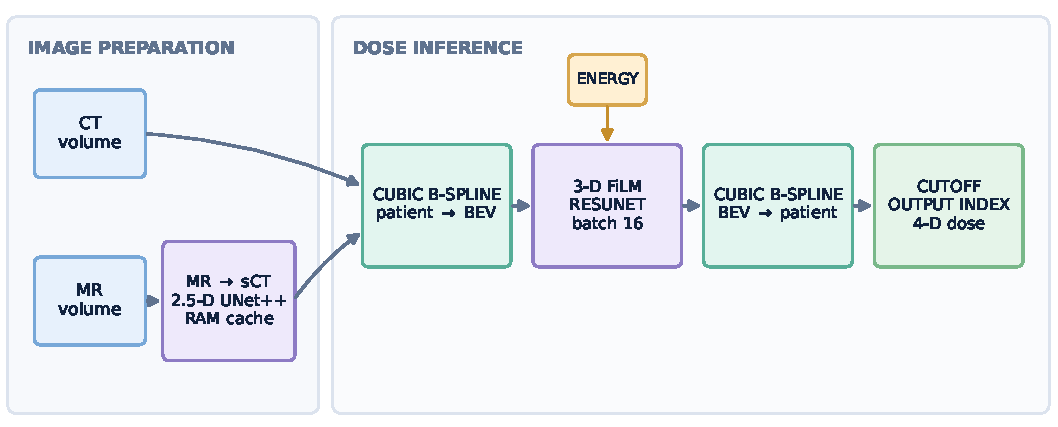
\includegraphics[width=\textwidth]{pipeline.pdf}
\caption{Final CT and MRI inference pipelines. The two task variants share the
same energy-conditioned dose model and patient--BEV transforms. The MRI branch
adds one in-memory sCT generation per unique image; no intermediate image is
written to disk.}
\label{fig:pipeline}
\end{figure}

\subsection{Beam-centered representation and dose network}

For a ray from source $\mathbf{s}$ to target $\mathbf{t}$, we formed an
orthonormal BEV frame from the propagation direction, a transverse lateral
axis, and the patient superior axis. The anatomical image was transformed with
an order-3 B-spline~\cite{unser1999splines} to a grid of
$288\times64\times64$ voxels (depth, lateral, superior) at
$2\times1\times1$~mm. Its first depth plane lies 320~mm upstream from
$\mathbf{t}$. Interpolated intensities were limited to the physical range
$[-1024,\max(I)]$ HU, then normalized as
\begin{equation}
 x=\frac{\mathrm{clip}(I,-1024,3000)+1024}{4024}.
\end{equation}
The array was quantized to float16 in the preprocessing cache and restored to
float32 by the training loader. Energy was mapped linearly from
[31.7290, 200.7966]~MeV to $[0,1]$.

The dose network, \methodname, is a residual 3-D U-Net derived from the
contracting/expanding design of U-Net~\cite{ronneberger2015unet}. Six feature
levels with base width six yield channel widths 6, 12, 24, 48, 96, and 192.
Each residual block contains two $3^3$ convolutions, GroupNorm
\cite{wu2018groupnorm}, SiLU, and an identity or $1^3$ projected skip. The
decoder uses trilinear upsampling, $1^3$ channel reduction, concatenation with
the encoder skip, and a residual block. Dropout3D of 0.05 is used at the
bottleneck and deepest decoder block.

A shared two-layer energy multilayer perceptron produces an embedding. Small
stage-specific heads apply residual feature-wise linear modulation
\cite{perez2018film}, $f'=f(1+\gamma)+\beta$, at encoder levels 3--5, the
bottleneck, and decoder levels
5--4. The FiLM heads were initialized to zero, hence to the identity. The final
$1^3$ head was initialized with standard deviation $10^{-3}$ and bias $-8$;
Softplus guarantees a non-negative BEV output. Training included two auxiliary
heads; after removing them, the deployed network has 3,094,511 trainable
parameters.

\subsection{MR-to-sCT model}

The MRI branch uses a 2.5-D UNet++~\cite{zhou2018unetplusplus} implemented with
Segmentation Models PyTorch. Five adjacent axial MR slices form the input and
the central CT slice is the target. The encoder is ResNet-34
\cite{he2016resnet}; the nested decoder and tanh head produce one normalized CT
slice. The 26,084,881-parameter model was initialized from ImpactSynth CV-1.

For each patient, the minimum and 99.5th percentile were computed on the full
MR volume, including background. Intensities were mapped to $[-1,1]$, clipped,
and stored as float16. Training crops were $320\times320$, centered on the body
bounding box for each nonempty slice. Two neighboring slices on either side
provided context; indices were reflected at the first and last slice. Values
outside the image were padded with $-1$.

At inference, the fully convolutional network processes each complete native
slice once. Height and width are padded once to a multiple of 32, and there is
no spatial tiling, stride, overlap, Gaussian importance map, or stitching.
Consequently, the Gaussian blending used in earlier experiments is not part of
the final pipeline. The normalized volume is uploaded once, five-slice
contexts are gathered on GPU, and slices are inferred in FP16 batches of 16.
Predictions are mapped to HU, clipped to $[-1024,3071]$, rounded to int16, and
voxels at which the original MR equals exactly zero are set to $-1024$ HU.
The MR and CT grids are already matched, so no sCT resampling is performed.

\subsection{Training}

Table~\ref{tab:training} summarizes the recorded configurations. The dose
target was multiplied globally by $10^5$ before float16 caching; predictions
were divided by the same constant at inference. Let $g_b$ and $p_b$ be the
ground-truth and predicted dose for beamlet $b$, $D_b=\max g_b$, and
$M_b=\{v:g_b(v)\geq0.1D_b\}$. The masked beam loss was
\begin{equation}
 \mathcal{L}_{\mathrm{MAE}}=
 \frac{1}{|M_b|D_b}\sum_{v\in M_b}|p_b(v)-g_b(v)|.
\end{equation}
The IDD loss summed dose over both transverse BEV axes and computed the RMS
difference of the depth curves after normalization by the maximum ground-truth
IDD. The main loss was
$\mathcal{L}_{\mathrm{dose}}=\mathcal{L}_{\mathrm{MAE}}+
\mathcal{L}_{\mathrm{IDD}}$. Auxiliary decoder heads used the same objective with weights 0.20
and 0.10 during training only; validation and inference used the main head.

The base dose model used AdamW~\cite{loshchilov2019adamw} with initial learning rate
$10^{-3}$ and weight decay $5\times10^{-4}$ on convolutional and linear
weights only. A cosine schedule targeted $2.5\times10^{-5}$ after 400 epochs.
The physical batch was two, with two-step gradient accumulation (effective
batch four), BF16 automatic mixed precision, gradient-norm clipping at 1.0,
and a deterministic cache without stochastic augmentation. The final 80-epoch
continuation started from the preceding phase's \texttt{last.pt}, retained
AdamW moments, scaler, and RNG state, and used a fresh cosine schedule from
$10^{-4}$ to $4\times10^{-5}$. Loss, batch, BF16, and clipping were unchanged;
paired CT--dose lateral flipping used $p=0.25$. Phase epoch 79 (stored as
zero-based epoch 78) minimized the main-head validation loss and was saved as
\texttt{best.pt}.

For sCT fine-tuning, the loss was
\begin{equation}
 \mathcal{L}_{\mathrm{sCT}}=\mathcal{L}_{1,\mathrm{body}}+
 0.15\,\mathcal{L}_{\mathrm{SAM}},
\end{equation}
where only L1 was masked and SAM-2.1-S-derived perceptual features
\cite{ravi2024sam2} were compared over the complete patch. AdamW parameter
groups used constant learning rates $10^{-5}$, $5\times10^{-5}$, and
$10^{-4}$ for encoder, decoder, and head, respectively, with weight decay
$10^{-3}$ and no scheduler. Training used FP16 mixed precision, batch 32,
32,000 samples (1,000 iterations) per epoch, and up to 50 epochs without early
stopping. Augmentation comprised horizontal flipping ($p=0.5$); a joint affine
transform ($p=0.35$, $\pm5^\circ$, $\pm10$ pixels); and MR-only intensity
augmentation ($p=0.5$) with gamma and gain in [0.9,1.1], bias in
[-0.08,0.08], and Gaussian-noise standard deviation in [0,0.025]. Vertical
flips were disabled. The final fold-1 checkpoint was epoch 6, selected by the
lowest mean per-patient validation body MAE.

\begin{table}[t]
\caption{Recorded configurations of the final dose phase and sCT model.}
\label{tab:training}
\centering
\small
\setlength{\tabcolsep}{3.2pt}
\begin{tabularx}{\textwidth}{@{}p{2.4cm}YY@{}}
\toprule
 & Dose model & MR-to-sCT model \\
\midrule
Architecture & Six-level FiLM residual 3-D U-Net, 3.09 M deployed parameters & 2.5-D UNet++/ResNet-34, 26.08 M parameters \\
Training input & $288\times64\times64$, spacing $2\times1\times1$ mm & Five $320\times320$ slices \\
Split & Final phase: 69 train; 6 monitored validation & 63 train; 12 representative validation \\
Loss & Masked beam MAE + IDD; auxiliary weights 0.20/0.10 & Body L1 + $0.15\,$SAM perceptual \\
Optimizer & AdamW, LR $10^{-4}$, WD $5\times10^{-4}$ (weights only) & AdamW, LRs $10^{-5}/5\times10^{-5}/10^{-4}$, WD $10^{-3}$ \\
Schedule & 80-epoch cosine to $4\times10^{-5}$ & None; constant learning rates \\
Batch/precision & 2, accumulation 2; BF16 AMP & 32; FP16 AMP \\
Augmentation & Paired lateral flip, $p=0.25$ & Flip, joint affine, MR intensity/noise \\
Final checkpoint & Continuation epoch 79, minimum validation loss & Fold 1 epoch 6, minimum validation body MAE \\
\bottomrule
\end{tabularx}
\end{table}

\subsection{Inference and output construction}

The two networks were loaded once during container startup, moved to GPU,
placed in evaluation mode, and warmed before the health endpoint became ready.
Inference used PyTorch inference mode, channels-last
layouts, and batch 16 for both dose and sCT. Dose used BF16 autocast when the
GPU supported it and FP16 otherwise; sCT used FP16. CuPy executed the spline
prefilter and affine transforms on GPU.

One spline prefilter was computed per anatomy. BEV anatomy was cached by exact
ray source and target, so the two energies on a ray reused the same volume.
For MRI, an LRU cache retained up to ten int16 sCTs in CPU RAM and reused an
sCT across Invoke calls when the same MR image and geometry recurred. No
temporary sCT files are created.

The predicted BEV dose was divided by $10^5$ and inverse-resampled with an
order-3 B-spline directly into a preallocated native-grid output buffer.
Negative cubic ringing was removed. For each beamlet, the challenge-supplied
\path{minimum_cutoff} field was applied inclusively,
$p_b(v)=0$ whenever $p_b(v)\leq c_b$. This cutoff is independent of the 10\%
ground-truth mask used by the evaluation metric. No upper dose clipping,
smoothing, amplitude calibration, or connected-component filtering was used.
Each frame was placed explicitly at its supplied output-file and frame indices;
ten compressed 4-D MetaImage stacks were written, including placeholders for
unused slots. Compression was performed concurrently with GPU computation.

\section{Evaluation}

Masked beam MAE in Eq.~(2) matches the current Level-1 source. However, its IDD
integrates along a fixed array axis (\texttt{beam\_axis=0}), whereas the
native-space report script calls an unavailable older direction-and-spacing
IDD interface. Its raw CT/MR reports are also absent. The results below are
therefore historical internal diagnostics pending recomputation with the
retained challenge evaluator. Metrics give beamlets equal weight within each
patient and patients equal weight overall.

The final checkpoint was selected by the minimum main-head composite loss on
the six cached-BEV validation patients. This surrogate uses the same MAE and
IDD definitions as training, but is not a native-space Level-1 evaluation.
The historical native-space CT evaluation used all 1,080 beamlets from each of
ten patients before four were moved into final training. The MRI diagnostic
used seven evenly spaced angles for each of the six dose-validation patients,
retaining all rays and energies (1,260 beamlets). These six also belonged to
sCT training, so the MRI result is not an independent sCT evaluation.

For sCT, body MAE was calculated inside a CT-derived mask: CT $>-900$ HU,
3-D binary closing, largest connected component, and hole filling. The
12-patient fold-1 validation was evaluated on reconstructed full volumes. On
the six dose patients we additionally computed PSNR with fixed 4,095-HU data
range and slice-wise Gaussian SSIM~\cite{wang2004ssim} ($\sigma=1.5$), averaged
inside the CT body. We report mean, population standard deviation (matching the
saved evaluator reports), median, and a two-sided 95\% Student-$t$ confidence
interval over patient means where available. These intervals quantify sampling
uncertainty of small internal cohorts, not external generalization.

To quantify the numerical cost of the coordinate transforms independently of
the network, we also retained an identity round-trip diagnostic: native
reference dose was projected to BEV, stored as float16, and reconstructed on
its original patient grid before masked beam MAE was computed. The proton
experiment used the final $288\times64\times64$, $2\times1\times1$-mm grid and
order-3 B-splines in both directions for all 10,800 beamlets of the historical
ten-patient cohort. An earlier seven-control-point photon diagnostic used a
$256\times200\times200$ isotropic 2-mm grid to compare cubic and linear
interpolation. The photon experiment therefore evaluates interpolation order
on a different grid; it is not an estimate of the final proton pipeline.

Runtime was reported through the actual HTTP Invoke path after model loading
and warm-up. The final dose continuation ran on one NVIDIA RTX 6000 Ada GPU
(48~GiB), with an Intel Xeon W5-3425 CPU and 502~GiB host RAM. The historical
HTTP profiler artifact is absent, so its workstation metadata cannot be
reverified. The documented Docker runtime used PyTorch 2.9.1, CUDA 12.6, CuPy
13.6, and SimpleITK 2.5.4.

\section{Results}

\subsection{Dose and sCT accuracy}

% TODO(camera-ready): replace the historical native-space table below with an
% evaluation of the final epoch-79 checkpoint using the retained evaluator.
The final continuation completed 80 epochs. Phase epoch 79 was selected as
\texttt{best.pt}, with cached-BEV validation loss 0.0108966 (masked MAE
0.0063354; IDD 0.0045612). These values are model-selection surrogates, not
native-space metrics. Table~\ref{tab:dose-results} therefore retains the
epoch-372 native-space results only as a pre-continuation reference. They must
not be interpreted as the final checkpoint's accuracy, particularly because
four of the ten CT cases subsequently entered final-phase training.

\begin{table}[t]
\caption{Historical pre-continuation native-space dose results; IDD requires
reconciliation with the current fixed-axis evaluator. Values are mean
$\pm$ population SD over patient means; CI is the two-sided 95\% Student-$t$
interval.}
\label{tab:dose-results}
\centering
\scriptsize
\setlength{\tabcolsep}{2.5pt}
\begin{tabular}{@{}llrrrr@{}}
\toprule
Task & Metric & Mean $\pm$ SD & Median & 95\% CI & Patients/beamlets \\
\midrule
CT & Masked beam MAE & .007958 $\pm$ .000687 & .007842 & [.007440,.008476] & 10/10,800 \\
CT & IDD distance & .007785 $\pm$ .001456 & .007592 & [.006687,.008882] & 10/10,800 \\
MR & Masked beam MAE & .011526 $\pm$ .000931 & .011903 & [.010456,.012596] & 6/1,260 \\
MR & IDD distance & .012500 $\pm$ .001413 & .012505 & [.010876,.014124] & 6/1,260 \\
\bottomrule
\end{tabular}
\end{table}

The historical sCT report for the independent 12-patient fold-1 validation set
gave a full-volume body MAE of $51.995\pm14.756$ HU (median 48.914, 95\% CI
[42.203,61.788]); values
ranged from 37.371 to 91.615 HU, with the largest error on thoracic patient
1THB031. On the six non-independent dose patients, the diagnostic body MAE,
SSIM, and PSNR were $38.366\pm3.831$ HU, $0.869776\pm0.016437$, and
$34.396\pm1.307$ dB. A representative thoracic slice is shown in
Fig.~\ref{fig:sct}.

\begin{figure}[t]
\centering
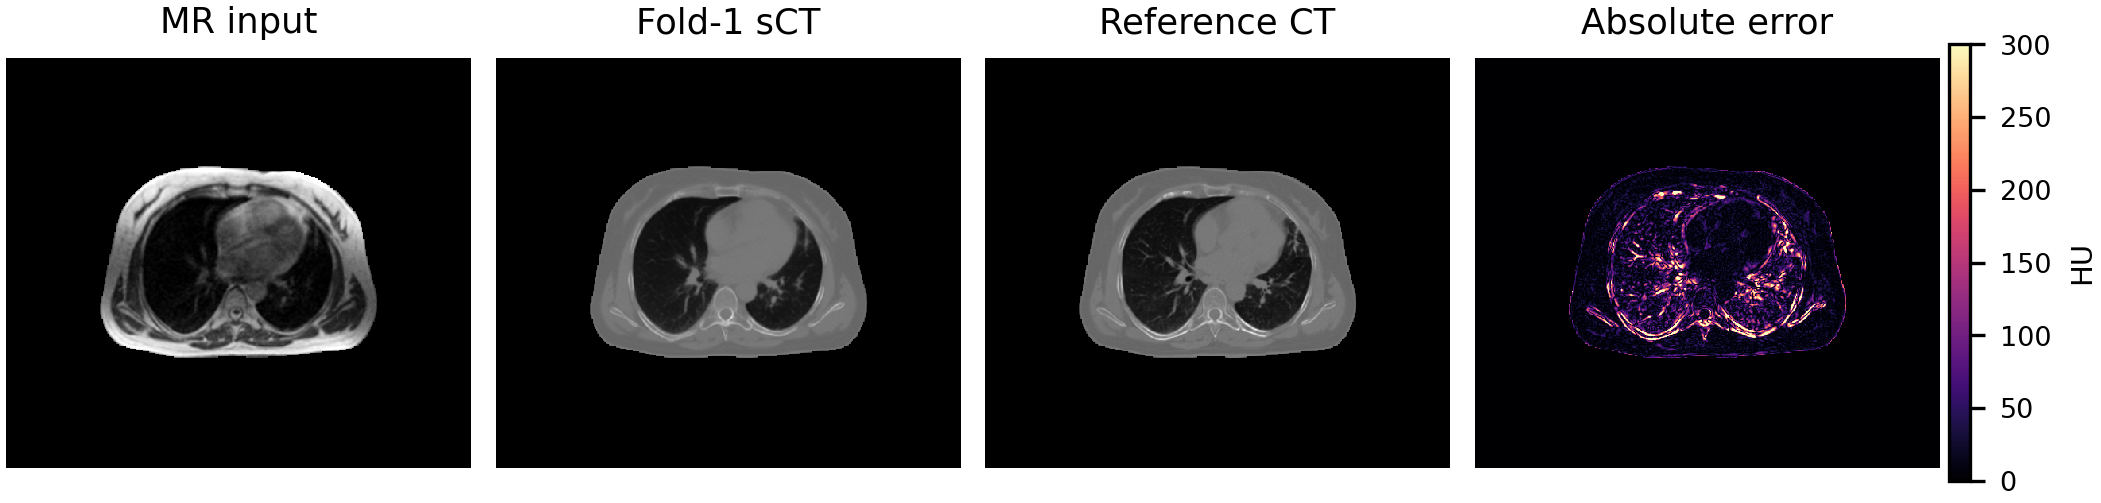
\includegraphics[width=0.94\textwidth]{qualitative_sct.png}
\caption{Diagnostic example from thoracic patient 1THB008. MR display limits
are its nonzero 1st--99th percentiles; CT and sCT use the same
[-1000,1200]-HU window, and absolute error is clipped at 300 HU for display.
This patient was in sCT fold-1 training and is shown qualitatively, not as an
independent test case.}
\label{fig:sct}
\end{figure}

\subsection{Patient--BEV round-trip diagnostic}

The proton identity round-trip gave masked beam MAE
$0.003264\pm0.000200$ (Table~\ref{tab:roundtrip}). This is not a strict lower
bound on prediction error because a network may compensate for systematic
effects. It jointly measures forward interpolation, float16 cache
quantization, and inverse interpolation, whose contributions cannot be
separated here. The ten-patient cohort predates the final continuation split;
four of these patients subsequently entered training.

\begin{table}[h]
\caption{Reference-dose round-trip masked beam MAE. Proton: mean $\pm$ SD of
patient means; photon: median [minimum, maximum].}
\label{tab:roundtrip}
\centering
\scriptsize
\setlength{\tabcolsep}{3pt}
\begin{tabular}{@{}lllll@{}}
\toprule
Data & Grid & Order & $n$ & Masked beam MAE \\
\midrule
Proton & $288\times64\times64$; $2\times1\times1$ mm & Cubic & 10/10,800 & $.003264\pm.000200$ \\
Photon & $256\times200\times200$; 2 mm & Cubic & 7 & $.006035$ [.003191,.011326] \\
Photon & $256\times200\times200$; 2 mm & Linear & 7 & $.017600$ [.012873,.034963] \\
\bottomrule
\end{tabular}
\end{table}

On the photon controls, the median linear round-trip error was 2.92 times the
cubic value. This diagnostic supports the retained order-3 interpolation, but
the cross-grid comparison is not a paired proton ablation.

\subsection{Single sCT model versus ensembles and postprocessing}

In the pre-continuation diagnostic on six patients and 1,260 beamlets,
three-fold averaging improved sCT MAE by 1.86\% but worsened both dose metrics
and approximately doubled sCT latency, so fold 1 alone was retained. Removing
the exact-zero MR air mask or applying Gaussian smoothing worsened HU MAE;
connected-component cleanup changed no voxels, while light dose smoothing had
negligible and inconsistent effects. None of these postprocessings was retained.

\subsection{Runtime}

Table~\ref{tab:runtime} reports a pre-continuation CT benchmark of the same
architecture and batch size: one
$590\times518\times146$ volume, 176 beamlets, and ten output stacks. Total
Invoke time was 7.9118~s (45.0~ms per beamlet). BEV-to-patient interpolation
remained the largest serial GPU/host stage. Compression CPU time totaled
7.1638~s but overlapped GPU work; writer waiting was 0.6605~s. Peak VRAM and
process RSS were 6.461 and 2.663~GiB.

Across the six MRI volumes, loaded-and-warmed fold-1 sCT generation averaged
1.265~s (median 1.395, maximum 1.681) at batch 16. The model forward averaged
0.647~s; normalization and HU conversion averaged 0.344 and 0.165~s. The sCT
cost is paid once per MR and amortized across its beamlets; a two-beamlet
integration fixture was therefore not considered a representative full case.

\begin{table}[h]
\caption{Historical local CT Invoke profile for 176 beamlets. Compression CPU
time overlaps other stages and is shown separately from critical-path writer
wait; the original profiler log must be restored for archival reproducibility.}
\label{tab:runtime}
\centering
\small
\begin{tabular}{@{}lr@{}}
\toprule
Component & Time (s) \\
\midrule
CT read & 0.3133 \\
Anatomy spline prefilter & 0.2989 \\
Anatomy-to-BEV projections & 0.0916 \\
Dose network (batch 16) & 1.8819 \\
BEV-to-patient interpolation & 4.4145 \\
Compression CPU work (overlapped) & 7.1638 \\
Writer wait on critical path & 0.6605 \\
\midrule
Complete Invoke & \textbf{7.9118} \\
\bottomrule
\end{tabular}
\end{table}

\section{Discussion}

The BEV representation lets a compact network learn range and lateral dose in
a normalized geometry. FiLM supplies energy at deep levels while early image
features remain shared across CT, MR, anatomies, and energies. Non-negativity
and the supplied per-beamlet cutoff impose explicit output constraints without
validation-fitted amplitude calibration.

The patient--BEV round-trip shows that interpolation is not lossless, while
the photon diagnostic found substantially lower error with cubic than linear
interpolation. This supports the retained order-3 transforms, without treating
the round-trip value as a strict lower bound. sCT ensembling improved HU MAE
but degraded dose and doubled latency, supporting the final single-model route.

All quantitative results are internal. Six CT patients were monitored during
dose training, and all six MRI dose patients entered sCT fine-tuning, making
the end-to-end MR result optimistic. The independent sCT fold had higher MAE,
including one 91.6-HU case. Moreover, public sCT pretraining used SynthRAD
2023/2025 data, while DoseRAD derives from SynthRAD2025.

The final dose checkpoint is continuation epoch 79, selected on six-patient
cached-BEV loss. Its native-space results remain unavailable, so the dose table
is explicitly a pre-continuation reference rather than final accuracy. Four CT
cases in that table entered final training. A representative full MRI Invoke
benchmark, raw reports, and beam/angle analysis are also unavailable.

Finally, the single-center cohort covers only thorax and abdomen with a
standardized MR acquisition. Scanner shifts, metal artifacts, other anatomies,
out-of-range energies, and clinical spot distributions remain untested. Hidden-
cohort and independent MR dose evaluation are required before clinical use.

\section*{Author Contributions (CRediT)}

\textbf{C\'edric H\'emon:} Conceptualization, Methodology, Software,
Validation, Formal analysis, Investigation, Writing (original draft).
\textbf{Valentin Boussot:} Methodology, Software, Writing (review \& editing).
\textbf{Jean-Claude Nunes:} Supervision, Writing (review \& editing).
\textbf{Caroline Lafond:} Supervision, Project administration, Writing (review \& editing).

\begin{credits}
\subsubsection{\discintname}
The authors have no competing interests to declare.
\end{credits}

\bibliographystyle{splncs04}
\bibliography{references}

\end{document}
